\section{Document Management System}

\subsection{Requirements}
The Contractor shall provide a Document Management System which includes the
ability to house electronically-filed court documents and auto-relate them to a
case index, the ability to scan images and auto-relate them to a case index,
the ability to apply digital annotations to imaged documents as part of agile
workflow, the ability to auto-post Orders created from the Judicial Dashboard
into the case index in real-time, and to keyword search and redact elements
inside digital images housed in the Document Management System.

\subsection{Breakdown}
\begin{itemize}
	\item Storage of electronic court documents
	\item indexing of court documents to a case, presumably with a
	pre-existing id
	\item ability to scan images
	\item automatically relate scans to case index
	\item apply digital annotations to imaged documents
	\item application of digital annotations must be part of
	agile\footnote{unclear what is meant by this}
	\item push orders from Judicial Dashboard into the case index
	\item keyword search
	\item redact elements of the scans
\end{itemize}

\subsection{Necessarily Implied By Requirements}
The requirement here seems to be an indexing system that needs to plug into an
existing id.  This sounds like an SQL DB tracking files in some kind of data
store.  Presumably there needs to be a way to track and apply edits, which will
imply some kind of frontend for interpreting edits.

\paragraph{Redactions}There also appears to be a request for some kind of
editor to ``apply redactions."  Generally, if redactions are required, we
should expect this to be firm and probably important.  This has security
implications.  How do we do a redaction that truly honors the requirement that
the information so redacted is actually inaccessible?  It seems to me that a
document server that serves this will need to store an original and apply
redactions \textbf{before} the file leaves the server.  This further implies
that the system will need some kind of authorization and some kind of access
level tracking.  It will need to be verifiably secure, as well.

\paragraph{Annotations}The requirement that digital annotations be applied to
an imaged document seems like a common-ish concept.  This clearly requires both
frontend support and backend support.  You will need a method for applying
annotations, and a method for capturing these annotations and associating them
with a particular digital document.  Typical annotations systems will tend to
offer a text box, which really boils down to a top-left position for the start
of the box, and a width.  The rest of the box would be implied by the amount of
text written.  This would probably constitute a simple version, and later
versions (if necessary) could then perhaps talk about such things as font and
point size.  This is only if we implement this ourselves, although given the
specific nature of system it seems like the sort of thing that would need to be
custom built.

\paragraph{Relation to Case Index}A number of these requirements allude to
association with a case index.  Presumeably this already exists, since it
sounds like something that the court is using to track cases that exist outside
the system and not mearly some nicety of an existing system.  However, this
charge is unclear, since it could mean anything from enter a case id into the
system to get an AI system to figure out what case ID is appropriate to ``gee
you have this case id open, why don't I associate this document you're adding
to this case id?"  Of the three possibilities, I consider the last possibility
to be the most likely.

In any case, it means at the very least that redactions, annotations, and
images must all refer to a case index, and that seems to be the central idea
they are trying to get across.

\paragraph{Keyword Search}The way this is phrased it sounds like what they want
is a way to keyword search scanned documents.  This would need to be an OCR
system.  Otherwise, if they are just trying to keyword search metadata and
annotations, this would be trivial.  Maybe this is indeed what they want?  In
any case, there are some IR packages out there that probably aren't too bad.  I
mean how, can you really do worse than MS Outlook?

\paragraph{Document Management System}It's not entirely clear what this is.  Is
this meant to be a service?  Or an application?  Or both?  My guess would be
both.

\subsection{Proposed Solution}
\begin{figure}[h]
	\begin{center}
		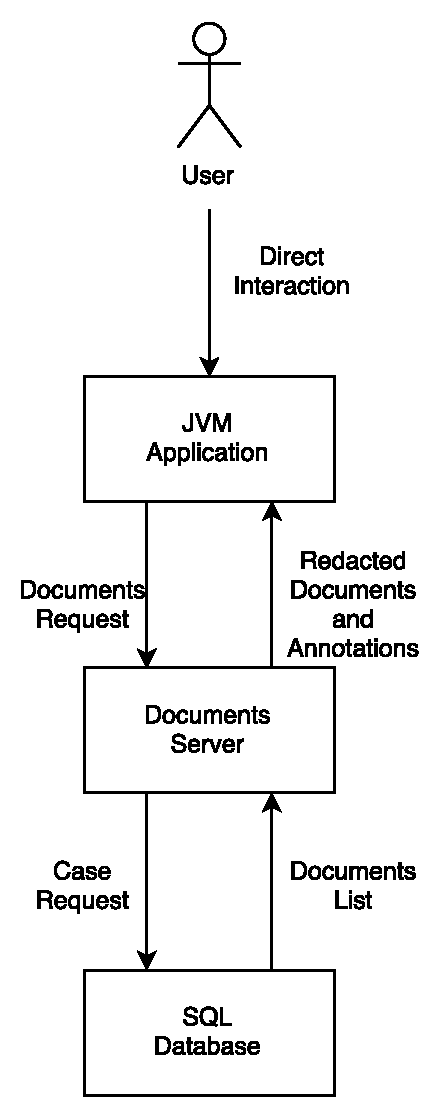
\includegraphics[scale=0.4]{images/DocumentManagementSystem.pdf}
	\end{center}
	\caption{High Level DMS Architecture}
	\label{fig:dmsArch}
\end{figure}

An overall solution would involve three main components:
\begin{itemize}
	\item a client application running on a user's laptop, desktop or other
		device in a JVM
	\item an sql document tracker running on a unix-compliant server.
	\item a document server running on a unix-compliant server.
\end{itemize}

\paragraph{Client Application}The client application would be the main view
into the system.  This would offer an interface for secure authentication, to
be validated by the SQL server and probably some layer on top of
it\footnote{what existing authentication solutions exist?}.  The function of
this application would be to display images retrieved by the rest of the
system, and to apply annotations correctly within the application to the user.

\paragraph{SQL Document Tracker}The document tracker would resolve which
documents are associated with which cases, and what access levels are
appropriate for each authenticated user given their enrollment in the system.
Once this document list is resolved, it can be sent to the document server,
which in turn will actually retrieve and transmit the documents to the client
application.

\paragraph{Document Management System}This subsystem will actually control the
documents, their annotations, and redaction deltas.  Given a list of documents,
it would apply redactions to images directly prior to sending, then pair the
resulting image with any annotations.  This process would be repeated for all
documents in the list, bundled together, and sent back to the requesting
client.

\paragraph{On second thought}Probably the jvm app would want to talk to the DMS
directly, and the DMS would talk to the SQL server.  It doesn't make any sense
for the DMS to trust the client app's word that the list it got was appropriate
for the authenticated user's access level.

\paragraph{Communications}It is in general possible to accomplish all said
communication with json-based rest calls.  For image data, byte streams are
allowed, although we would probably want to do something like base-64 encoding
to return the image data.
